% Options for packages loaded elsewhere
\PassOptionsToPackage{unicode}{hyperref}
\PassOptionsToPackage{hyphens}{url}
%
\documentclass[
]{article}
\usepackage{lmodern}
\usepackage{amssymb,amsmath}
\usepackage{ifxetex,ifluatex}
\ifnum 0\ifxetex 1\fi\ifluatex 1\fi=0 % if pdftex
  \usepackage[T1]{fontenc}
  \usepackage[utf8]{inputenc}
  \usepackage{textcomp} % provide euro and other symbols
\else % if luatex or xetex
  \usepackage{unicode-math}
  \defaultfontfeatures{Scale=MatchLowercase}
  \defaultfontfeatures[\rmfamily]{Ligatures=TeX,Scale=1}
\fi
% Use upquote if available, for straight quotes in verbatim environments
\IfFileExists{upquote.sty}{\usepackage{upquote}}{}
\IfFileExists{microtype.sty}{% use microtype if available
  \usepackage[]{microtype}
  \UseMicrotypeSet[protrusion]{basicmath} % disable protrusion for tt fonts
}{}
\makeatletter
\@ifundefined{KOMAClassName}{% if non-KOMA class
  \IfFileExists{parskip.sty}{%
    \usepackage{parskip}
  }{% else
    \setlength{\parindent}{0pt}
    \setlength{\parskip}{6pt plus 2pt minus 1pt}}
}{% if KOMA class
  \KOMAoptions{parskip=half}}
\makeatother
\usepackage{xcolor}
\IfFileExists{xurl.sty}{\usepackage{xurl}}{} % add URL line breaks if available
\IfFileExists{bookmark.sty}{\usepackage{bookmark}}{\usepackage{hyperref}}
\hypersetup{
  hidelinks,
  pdfcreator={LaTeX via pandoc}}
\urlstyle{same} % disable monospaced font for URLs
\usepackage[margin=1in]{geometry}
\usepackage{color}
\usepackage{fancyvrb}
\newcommand{\VerbBar}{|}
\newcommand{\VERB}{\Verb[commandchars=\\\{\}]}
\DefineVerbatimEnvironment{Highlighting}{Verbatim}{commandchars=\\\{\}}
% Add ',fontsize=\small' for more characters per line
\usepackage{framed}
\definecolor{shadecolor}{RGB}{248,248,248}
\newenvironment{Shaded}{\begin{snugshade}}{\end{snugshade}}
\newcommand{\AlertTok}[1]{\textcolor[rgb]{0.94,0.16,0.16}{#1}}
\newcommand{\AnnotationTok}[1]{\textcolor[rgb]{0.56,0.35,0.01}{\textbf{\textit{#1}}}}
\newcommand{\AttributeTok}[1]{\textcolor[rgb]{0.77,0.63,0.00}{#1}}
\newcommand{\BaseNTok}[1]{\textcolor[rgb]{0.00,0.00,0.81}{#1}}
\newcommand{\BuiltInTok}[1]{#1}
\newcommand{\CharTok}[1]{\textcolor[rgb]{0.31,0.60,0.02}{#1}}
\newcommand{\CommentTok}[1]{\textcolor[rgb]{0.56,0.35,0.01}{\textit{#1}}}
\newcommand{\CommentVarTok}[1]{\textcolor[rgb]{0.56,0.35,0.01}{\textbf{\textit{#1}}}}
\newcommand{\ConstantTok}[1]{\textcolor[rgb]{0.00,0.00,0.00}{#1}}
\newcommand{\ControlFlowTok}[1]{\textcolor[rgb]{0.13,0.29,0.53}{\textbf{#1}}}
\newcommand{\DataTypeTok}[1]{\textcolor[rgb]{0.13,0.29,0.53}{#1}}
\newcommand{\DecValTok}[1]{\textcolor[rgb]{0.00,0.00,0.81}{#1}}
\newcommand{\DocumentationTok}[1]{\textcolor[rgb]{0.56,0.35,0.01}{\textbf{\textit{#1}}}}
\newcommand{\ErrorTok}[1]{\textcolor[rgb]{0.64,0.00,0.00}{\textbf{#1}}}
\newcommand{\ExtensionTok}[1]{#1}
\newcommand{\FloatTok}[1]{\textcolor[rgb]{0.00,0.00,0.81}{#1}}
\newcommand{\FunctionTok}[1]{\textcolor[rgb]{0.00,0.00,0.00}{#1}}
\newcommand{\ImportTok}[1]{#1}
\newcommand{\InformationTok}[1]{\textcolor[rgb]{0.56,0.35,0.01}{\textbf{\textit{#1}}}}
\newcommand{\KeywordTok}[1]{\textcolor[rgb]{0.13,0.29,0.53}{\textbf{#1}}}
\newcommand{\NormalTok}[1]{#1}
\newcommand{\OperatorTok}[1]{\textcolor[rgb]{0.81,0.36,0.00}{\textbf{#1}}}
\newcommand{\OtherTok}[1]{\textcolor[rgb]{0.56,0.35,0.01}{#1}}
\newcommand{\PreprocessorTok}[1]{\textcolor[rgb]{0.56,0.35,0.01}{\textit{#1}}}
\newcommand{\RegionMarkerTok}[1]{#1}
\newcommand{\SpecialCharTok}[1]{\textcolor[rgb]{0.00,0.00,0.00}{#1}}
\newcommand{\SpecialStringTok}[1]{\textcolor[rgb]{0.31,0.60,0.02}{#1}}
\newcommand{\StringTok}[1]{\textcolor[rgb]{0.31,0.60,0.02}{#1}}
\newcommand{\VariableTok}[1]{\textcolor[rgb]{0.00,0.00,0.00}{#1}}
\newcommand{\VerbatimStringTok}[1]{\textcolor[rgb]{0.31,0.60,0.02}{#1}}
\newcommand{\WarningTok}[1]{\textcolor[rgb]{0.56,0.35,0.01}{\textbf{\textit{#1}}}}
\usepackage{graphicx,grffile}
\makeatletter
\def\maxwidth{\ifdim\Gin@nat@width>\linewidth\linewidth\else\Gin@nat@width\fi}
\def\maxheight{\ifdim\Gin@nat@height>\textheight\textheight\else\Gin@nat@height\fi}
\makeatother
% Scale images if necessary, so that they will not overflow the page
% margins by default, and it is still possible to overwrite the defaults
% using explicit options in \includegraphics[width, height, ...]{}
\setkeys{Gin}{width=\maxwidth,height=\maxheight,keepaspectratio}
% Set default figure placement to htbp
\makeatletter
\def\fps@figure{htbp}
\makeatother
\setlength{\emergencystretch}{3em} % prevent overfull lines
\providecommand{\tightlist}{%
  \setlength{\itemsep}{0pt}\setlength{\parskip}{0pt}}
\setcounter{secnumdepth}{-\maxdimen} % remove section numbering

\author{}
\date{\vspace{-2.5em}}

\begin{document}

\begin{Shaded}
\begin{Highlighting}[]
\CommentTok{#2.}

\KeywordTok{library}\NormalTok{(MASS)}
\KeywordTok{data}\NormalTok{(}\StringTok{"Boston"}\NormalTok{)}

\KeywordTok{str}\NormalTok{(Boston)}
\end{Highlighting}
\end{Shaded}

\begin{verbatim}
## 'data.frame':    506 obs. of  14 variables:
##  $ crim   : num  0.00632 0.02731 0.02729 0.03237 0.06905 ...
##  $ zn     : num  18 0 0 0 0 0 12.5 12.5 12.5 12.5 ...
##  $ indus  : num  2.31 7.07 7.07 2.18 2.18 2.18 7.87 7.87 7.87 7.87 ...
##  $ chas   : int  0 0 0 0 0 0 0 0 0 0 ...
##  $ nox    : num  0.538 0.469 0.469 0.458 0.458 0.458 0.524 0.524 0.524 0.524 ...
##  $ rm     : num  6.58 6.42 7.18 7 7.15 ...
##  $ age    : num  65.2 78.9 61.1 45.8 54.2 58.7 66.6 96.1 100 85.9 ...
##  $ dis    : num  4.09 4.97 4.97 6.06 6.06 ...
##  $ rad    : int  1 2 2 3 3 3 5 5 5 5 ...
##  $ tax    : num  296 242 242 222 222 222 311 311 311 311 ...
##  $ ptratio: num  15.3 17.8 17.8 18.7 18.7 18.7 15.2 15.2 15.2 15.2 ...
##  $ black  : num  397 397 393 395 397 ...
##  $ lstat  : num  4.98 9.14 4.03 2.94 5.33 ...
##  $ medv   : num  24 21.6 34.7 33.4 36.2 28.7 22.9 27.1 16.5 18.9 ...
\end{verbatim}

\begin{Shaded}
\begin{Highlighting}[]
\KeywordTok{dim}\NormalTok{(Boston)}
\end{Highlighting}
\end{Shaded}

\begin{verbatim}
## [1] 506  14
\end{verbatim}

\begin{Shaded}
\begin{Highlighting}[]
\NormalTok{testi=}\StringTok{ }\KeywordTok{cbind}\NormalTok{(Boston[}\DecValTok{1}\OperatorTok{:}\DecValTok{2}\NormalTok{], Boston[}\DecValTok{3}\NormalTok{])}

\NormalTok{testaa=}\StringTok{ }\NormalTok{testi[}\KeywordTok{c}\NormalTok{(}\DecValTok{3}\NormalTok{, }\DecValTok{1}\OperatorTok{:}\DecValTok{2}\NormalTok{)]}
\end{Highlighting}
\end{Shaded}

\begin{Shaded}
\begin{Highlighting}[]
\CommentTok{#3.}

\KeywordTok{library}\NormalTok{(corrplot)}
\end{Highlighting}
\end{Shaded}

\begin{verbatim}
## corrplot 0.84 loaded
\end{verbatim}

\begin{Shaded}
\begin{Highlighting}[]
\KeywordTok{library}\NormalTok{(tidyverse)}
\end{Highlighting}
\end{Shaded}

\begin{verbatim}
## -- Attaching packages ----------------------------- tidyverse 1.3.0 --
\end{verbatim}

\begin{verbatim}
## v ggplot2 3.3.2     v purrr   0.3.4
## v tibble  3.0.3     v dplyr   1.0.2
## v tidyr   1.1.2     v stringr 1.4.0
## v readr   1.4.0     v forcats 0.5.0
\end{verbatim}

\begin{verbatim}
## -- Conflicts -------------------------------- tidyverse_conflicts() --
## x dplyr::filter() masks stats::filter()
## x dplyr::lag()    masks stats::lag()
## x dplyr::select() masks MASS::select()
\end{verbatim}

\begin{Shaded}
\begin{Highlighting}[]
\KeywordTok{pairs}\NormalTok{(Boston)}
\end{Highlighting}
\end{Shaded}

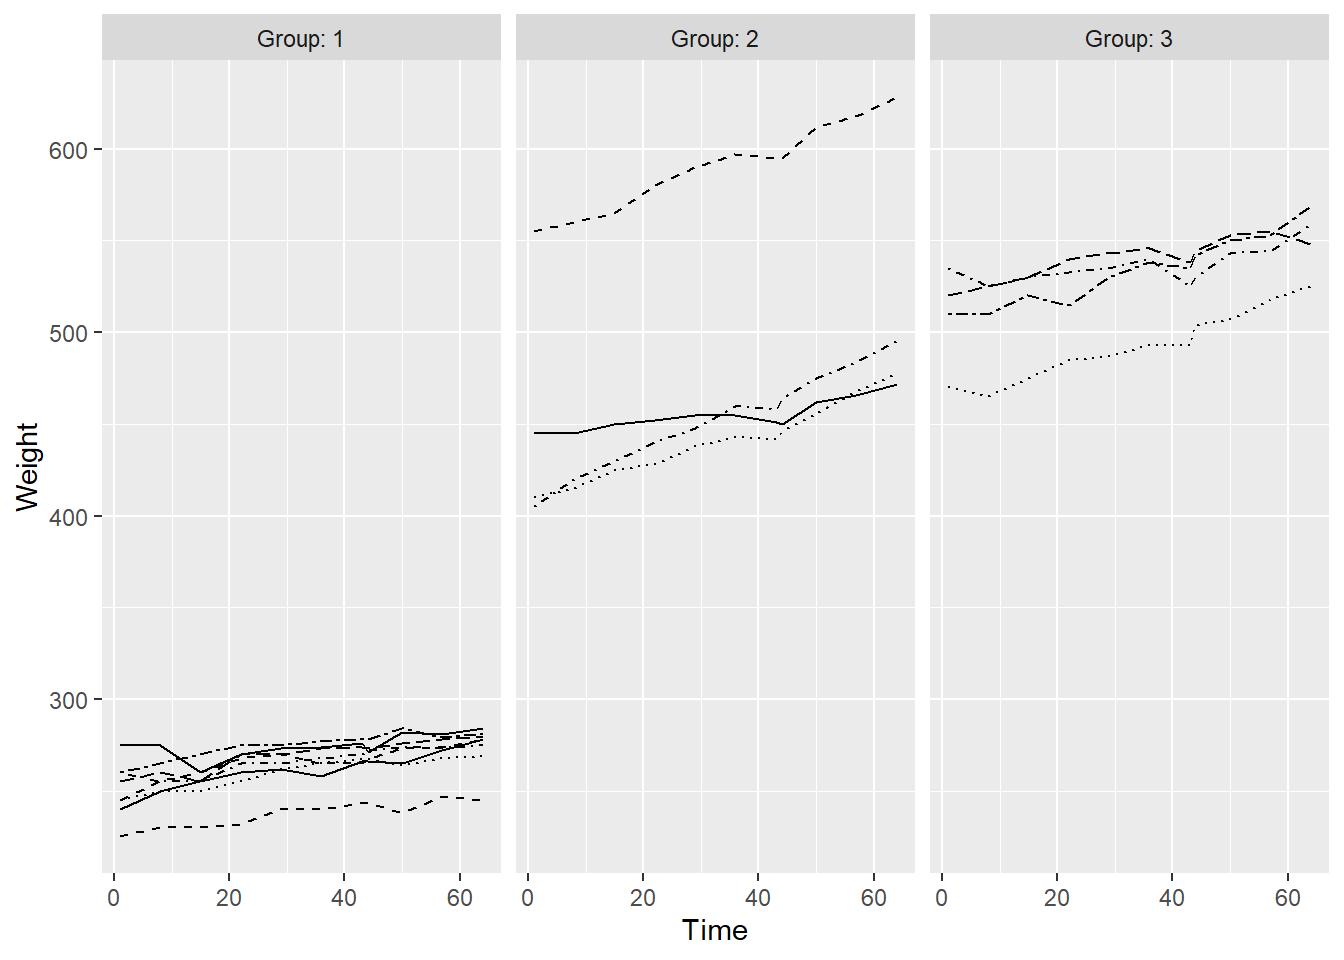
\includegraphics{chapter4_files/figure-latex/unnamed-chunk-2-1.pdf}

\begin{Shaded}
\begin{Highlighting}[]
\CommentTok{# calculate the correlation matrix and round it}
\NormalTok{cor_matrix<-}\KeywordTok{cor}\NormalTok{(Boston) }\OperatorTok
\KeywordTok{round}\NormalTok{(.,}\DecValTok{2}\NormalTok{)}
\NormalTok{cor_matrix}
\end{Highlighting}
\end{Shaded}

\begin{verbatim}
##          crim    zn indus  chas   nox    rm   age   dis   rad   tax ptratio
## crim     1.00 -0.20  0.41 -0.06  0.42 -0.22  0.35 -0.38  0.63  0.58    0.29
## zn      -0.20  1.00 -0.53 -0.04 -0.52  0.31 -0.57  0.66 -0.31 -0.31   -0.39
## indus    0.41 -0.53  1.00  0.06  0.76 -0.39  0.64 -0.71  0.60  0.72    0.38
## chas    -0.06 -0.04  0.06  1.00  0.09  0.09  0.09 -0.10 -0.01 -0.04   -0.12
## nox      0.42 -0.52  0.76  0.09  1.00 -0.30  0.73 -0.77  0.61  0.67    0.19
## rm      -0.22  0.31 -0.39  0.09 -0.30  1.00 -0.24  0.21 -0.21 -0.29   -0.36
## age      0.35 -0.57  0.64  0.09  0.73 -0.24  1.00 -0.75  0.46  0.51    0.26
## dis     -0.38  0.66 -0.71 -0.10 -0.77  0.21 -0.75  1.00 -0.49 -0.53   -0.23
## rad      0.63 -0.31  0.60 -0.01  0.61 -0.21  0.46 -0.49  1.00  0.91    0.46
## tax      0.58 -0.31  0.72 -0.04  0.67 -0.29  0.51 -0.53  0.91  1.00    0.46
## ptratio  0.29 -0.39  0.38 -0.12  0.19 -0.36  0.26 -0.23  0.46  0.46    1.00
## black   -0.39  0.18 -0.36  0.05 -0.38  0.13 -0.27  0.29 -0.44 -0.44   -0.18
## lstat    0.46 -0.41  0.60 -0.05  0.59 -0.61  0.60 -0.50  0.49  0.54    0.37
## medv    -0.39  0.36 -0.48  0.18 -0.43  0.70 -0.38  0.25 -0.38 -0.47   -0.51
##         black lstat  medv
## crim    -0.39  0.46 -0.39
## zn       0.18 -0.41  0.36
## indus   -0.36  0.60 -0.48
## chas     0.05 -0.05  0.18
## nox     -0.38  0.59 -0.43
## rm       0.13 -0.61  0.70
## age     -0.27  0.60 -0.38
## dis      0.29 -0.50  0.25
## rad     -0.44  0.49 -0.38
## tax     -0.44  0.54 -0.47
## ptratio -0.18  0.37 -0.51
## black    1.00 -0.37  0.33
## lstat   -0.37  1.00 -0.74
## medv     0.33 -0.74  1.00
\end{verbatim}

\begin{Shaded}
\begin{Highlighting}[]
\CommentTok{# print the correlation matrix}


\CommentTok{# visualize the correlation matrix}
\KeywordTok{corrplot}\NormalTok{(cor_matrix, }\DataTypeTok{method=}\StringTok{"circle"}\NormalTok{, }\DataTypeTok{type=} \StringTok{"upper"}\NormalTok{, }\DataTypeTok{cl.pos=} \StringTok{"b"}\NormalTok{, }\DataTypeTok{tl.pos=} \StringTok{"d"}\NormalTok{, }\DataTypeTok{tl.cex=} \FloatTok{0.6}\NormalTok{)}
\end{Highlighting}
\end{Shaded}

\includegraphics{chapter4_files/figure-latex/unnamed-chunk-2-2.pdf}

\begin{Shaded}
\begin{Highlighting}[]
\CommentTok{#4.}
\CommentTok{# center and standardize variables}

\KeywordTok{str}\NormalTok{(Boston)}
\end{Highlighting}
\end{Shaded}

\begin{verbatim}
## 'data.frame':    506 obs. of  14 variables:
##  $ crim   : num  0.00632 0.02731 0.02729 0.03237 0.06905 ...
##  $ zn     : num  18 0 0 0 0 0 12.5 12.5 12.5 12.5 ...
##  $ indus  : num  2.31 7.07 7.07 2.18 2.18 2.18 7.87 7.87 7.87 7.87 ...
##  $ chas   : int  0 0 0 0 0 0 0 0 0 0 ...
##  $ nox    : num  0.538 0.469 0.469 0.458 0.458 0.458 0.524 0.524 0.524 0.524 ...
##  $ rm     : num  6.58 6.42 7.18 7 7.15 ...
##  $ age    : num  65.2 78.9 61.1 45.8 54.2 58.7 66.6 96.1 100 85.9 ...
##  $ dis    : num  4.09 4.97 4.97 6.06 6.06 ...
##  $ rad    : int  1 2 2 3 3 3 5 5 5 5 ...
##  $ tax    : num  296 242 242 222 222 222 311 311 311 311 ...
##  $ ptratio: num  15.3 17.8 17.8 18.7 18.7 18.7 15.2 15.2 15.2 15.2 ...
##  $ black  : num  397 397 393 395 397 ...
##  $ lstat  : num  4.98 9.14 4.03 2.94 5.33 ...
##  $ medv   : num  24 21.6 34.7 33.4 36.2 28.7 22.9 27.1 16.5 18.9 ...
\end{verbatim}

\begin{Shaded}
\begin{Highlighting}[]
\NormalTok{boston_scaled <-}\StringTok{ }\KeywordTok{scale}\NormalTok{(Boston)}
\KeywordTok{str}\NormalTok{(boston_scaled)}
\end{Highlighting}
\end{Shaded}

\begin{verbatim}
##  num [1:506, 1:14] -0.419 -0.417 -0.417 -0.416 -0.412 ...
##  - attr(*, "dimnames")=List of 2
##   ..$ : chr [1:506] "1" "2" "3" "4" ...
##   ..$ : chr [1:14] "crim" "zn" "indus" "chas" ...
##  - attr(*, "scaled:center")= Named num [1:14] 3.6135 11.3636 11.1368 0.0692 0.5547 ...
##   ..- attr(*, "names")= chr [1:14] "crim" "zn" "indus" "chas" ...
##  - attr(*, "scaled:scale")= Named num [1:14] 8.602 23.322 6.86 0.254 0.116 ...
##   ..- attr(*, "names")= chr [1:14] "crim" "zn" "indus" "chas" ...
\end{verbatim}

\begin{Shaded}
\begin{Highlighting}[]
\CommentTok{# summaries of the scaled variables}
\KeywordTok{summary}\NormalTok{(boston_scaled)}
\end{Highlighting}
\end{Shaded}

\begin{verbatim}
##       crim                 zn               indus              chas        
##  Min.   :-0.419367   Min.   :-0.48724   Min.   :-1.5563   Min.   :-0.2723  
##  1st Qu.:-0.410563   1st Qu.:-0.48724   1st Qu.:-0.8668   1st Qu.:-0.2723  
##  Median :-0.390280   Median :-0.48724   Median :-0.2109   Median :-0.2723  
##  Mean   : 0.000000   Mean   : 0.00000   Mean   : 0.0000   Mean   : 0.0000  
##  3rd Qu.: 0.007389   3rd Qu.: 0.04872   3rd Qu.: 1.0150   3rd Qu.:-0.2723  
##  Max.   : 9.924110   Max.   : 3.80047   Max.   : 2.4202   Max.   : 3.6648  
##       nox                rm               age               dis         
##  Min.   :-1.4644   Min.   :-3.8764   Min.   :-2.3331   Min.   :-1.2658  
##  1st Qu.:-0.9121   1st Qu.:-0.5681   1st Qu.:-0.8366   1st Qu.:-0.8049  
##  Median :-0.1441   Median :-0.1084   Median : 0.3171   Median :-0.2790  
##  Mean   : 0.0000   Mean   : 0.0000   Mean   : 0.0000   Mean   : 0.0000  
##  3rd Qu.: 0.5981   3rd Qu.: 0.4823   3rd Qu.: 0.9059   3rd Qu.: 0.6617  
##  Max.   : 2.7296   Max.   : 3.5515   Max.   : 1.1164   Max.   : 3.9566  
##       rad               tax             ptratio            black        
##  Min.   :-0.9819   Min.   :-1.3127   Min.   :-2.7047   Min.   :-3.9033  
##  1st Qu.:-0.6373   1st Qu.:-0.7668   1st Qu.:-0.4876   1st Qu.: 0.2049  
##  Median :-0.5225   Median :-0.4642   Median : 0.2746   Median : 0.3808  
##  Mean   : 0.0000   Mean   : 0.0000   Mean   : 0.0000   Mean   : 0.0000  
##  3rd Qu.: 1.6596   3rd Qu.: 1.5294   3rd Qu.: 0.8058   3rd Qu.: 0.4332  
##  Max.   : 1.6596   Max.   : 1.7964   Max.   : 1.6372   Max.   : 0.4406  
##      lstat              medv        
##  Min.   :-1.5296   Min.   :-1.9063  
##  1st Qu.:-0.7986   1st Qu.:-0.5989  
##  Median :-0.1811   Median :-0.1449  
##  Mean   : 0.0000   Mean   : 0.0000  
##  3rd Qu.: 0.6024   3rd Qu.: 0.2683  
##  Max.   : 3.5453   Max.   : 2.9865
\end{verbatim}

\begin{Shaded}
\begin{Highlighting}[]
\CommentTok{# class of the boston_scaled object}
\KeywordTok{class}\NormalTok{(boston_scaled)}
\end{Highlighting}
\end{Shaded}

\begin{verbatim}
## [1] "matrix" "array"
\end{verbatim}

\begin{Shaded}
\begin{Highlighting}[]
\CommentTok{# change the object to data frame}
\NormalTok{boston_scaled =}\StringTok{ }\KeywordTok{as.data.frame}\NormalTok{(boston_scaled)}

\KeywordTok{str}\NormalTok{(boston_scaled)}
\end{Highlighting}
\end{Shaded}

\begin{verbatim}
## 'data.frame':    506 obs. of  14 variables:
##  $ crim   : num  -0.419 -0.417 -0.417 -0.416 -0.412 ...
##  $ zn     : num  0.285 -0.487 -0.487 -0.487 -0.487 ...
##  $ indus  : num  -1.287 -0.593 -0.593 -1.306 -1.306 ...
##  $ chas   : num  -0.272 -0.272 -0.272 -0.272 -0.272 ...
##  $ nox    : num  -0.144 -0.74 -0.74 -0.834 -0.834 ...
##  $ rm     : num  0.413 0.194 1.281 1.015 1.227 ...
##  $ age    : num  -0.12 0.367 -0.266 -0.809 -0.511 ...
##  $ dis    : num  0.14 0.557 0.557 1.077 1.077 ...
##  $ rad    : num  -0.982 -0.867 -0.867 -0.752 -0.752 ...
##  $ tax    : num  -0.666 -0.986 -0.986 -1.105 -1.105 ...
##  $ ptratio: num  -1.458 -0.303 -0.303 0.113 0.113 ...
##  $ black  : num  0.441 0.441 0.396 0.416 0.441 ...
##  $ lstat  : num  -1.074 -0.492 -1.208 -1.36 -1.025 ...
##  $ medv   : num  0.16 -0.101 1.323 1.182 1.486 ...
\end{verbatim}

\begin{Shaded}
\begin{Highlighting}[]
\CommentTok{# 6.}


\CommentTok{# boston_scaled is available}

\CommentTok{# save the scaled crim as scaled_crim}
\NormalTok{scaled_crim <-}\StringTok{ }\NormalTok{boston_scaled}\OperatorTok{$}\NormalTok{crim}

\CommentTok{# summary of the scaled_crim}
\KeywordTok{summary}\NormalTok{(scaled_crim)}
\end{Highlighting}
\end{Shaded}

\begin{verbatim}
##      Min.   1st Qu.    Median      Mean   3rd Qu.      Max. 
## -0.419367 -0.410563 -0.390280  0.000000  0.007389  9.924110
\end{verbatim}

\begin{Shaded}
\begin{Highlighting}[]
\CommentTok{# create a quantile vector of crim and print it}
\NormalTok{bins <-}\StringTok{ }\KeywordTok{quantile}\NormalTok{(scaled_crim)}
\NormalTok{bins}
\end{Highlighting}
\end{Shaded}

\begin{verbatim}
##           0%          25%          50%          75%         100% 
## -0.419366929 -0.410563278 -0.390280295  0.007389247  9.924109610
\end{verbatim}

\begin{Shaded}
\begin{Highlighting}[]
\KeywordTok{str}\NormalTok{(scaled_crim)}
\end{Highlighting}
\end{Shaded}

\begin{verbatim}
##  num [1:506] -0.419 -0.417 -0.417 -0.416 -0.412 ...
\end{verbatim}

\begin{Shaded}
\begin{Highlighting}[]
\CommentTok{# create a categorical variable 'crime'}
\NormalTok{crime <-}\StringTok{ }\KeywordTok{cut}\NormalTok{(scaled_crim, }\DataTypeTok{breaks =}\NormalTok{ bins, }\DataTypeTok{include.lowest =} \OtherTok{TRUE}\NormalTok{, labels}
\NormalTok{=}\KeywordTok{c}\NormalTok{(}\StringTok{"low"}\NormalTok{, }\StringTok{"med_low"}\NormalTok{, }\StringTok{"med_high"}\NormalTok{, }\StringTok{"high"}\NormalTok{))}

\CommentTok{# look at the table of the new factor crime}
\KeywordTok{table}\NormalTok{(crime)}
\end{Highlighting}
\end{Shaded}

\begin{verbatim}
## crime
##      low  med_low med_high     high 
##      127      126      126      127
\end{verbatim}

\begin{Shaded}
\begin{Highlighting}[]
\CommentTok{# remove original crim from the dataset}
\NormalTok{boston_scaled <-}\StringTok{ }\NormalTok{dplyr}\OperatorTok{::}\KeywordTok{select}\NormalTok{(boston_scaled, }\OperatorTok{-}\NormalTok{crim)}

\CommentTok{# add the new categorical value to scaled data}
\NormalTok{boston_scaled <-}\StringTok{ }\KeywordTok{data.frame}\NormalTok{(boston_scaled, crime)}

\CommentTok{# number of rows in the Boston dataset }
\NormalTok{n <-}\StringTok{ }\KeywordTok{nrow}\NormalTok{(boston_scaled)}

\CommentTok{# choose randomly 80% of the rows}
\NormalTok{ind <-}\StringTok{ }\KeywordTok{sample}\NormalTok{(n,  }\DataTypeTok{size =}\NormalTok{ n }\OperatorTok{*}\StringTok{ }\FloatTok{0.8}\NormalTok{)}

\CommentTok{# create train set}
\NormalTok{train <-}\StringTok{ }\NormalTok{boston_scaled[ind,]}

\CommentTok{# create test set }
\NormalTok{test <-}\StringTok{ }\NormalTok{boston_scaled[}\OperatorTok{-}\NormalTok{ind,]}

\CommentTok{# save the correct classes from test data}
\NormalTok{correct_classes <-}\StringTok{ }\NormalTok{test}\OperatorTok{$}\NormalTok{crime}

\CommentTok{# remove the crime variable from test data}
\NormalTok{test <-}\StringTok{ }\NormalTok{dplyr}\OperatorTok{::}\KeywordTok{select}\NormalTok{(test, }\OperatorTok{-}\NormalTok{crime)}

\KeywordTok{str}\NormalTok{(Boston)}
\end{Highlighting}
\end{Shaded}

\begin{verbatim}
## 'data.frame':    506 obs. of  14 variables:
##  $ crim   : num  0.00632 0.02731 0.02729 0.03237 0.06905 ...
##  $ zn     : num  18 0 0 0 0 0 12.5 12.5 12.5 12.5 ...
##  $ indus  : num  2.31 7.07 7.07 2.18 2.18 2.18 7.87 7.87 7.87 7.87 ...
##  $ chas   : int  0 0 0 0 0 0 0 0 0 0 ...
##  $ nox    : num  0.538 0.469 0.469 0.458 0.458 0.458 0.524 0.524 0.524 0.524 ...
##  $ rm     : num  6.58 6.42 7.18 7 7.15 ...
##  $ age    : num  65.2 78.9 61.1 45.8 54.2 58.7 66.6 96.1 100 85.9 ...
##  $ dis    : num  4.09 4.97 4.97 6.06 6.06 ...
##  $ rad    : int  1 2 2 3 3 3 5 5 5 5 ...
##  $ tax    : num  296 242 242 222 222 222 311 311 311 311 ...
##  $ ptratio: num  15.3 17.8 17.8 18.7 18.7 18.7 15.2 15.2 15.2 15.2 ...
##  $ black  : num  397 397 393 395 397 ...
##  $ lstat  : num  4.98 9.14 4.03 2.94 5.33 ...
##  $ medv   : num  24 21.6 34.7 33.4 36.2 28.7 22.9 27.1 16.5 18.9 ...
\end{verbatim}

\begin{Shaded}
\begin{Highlighting}[]
\NormalTok{lda.fit <-}\StringTok{ }\KeywordTok{lda}\NormalTok{(crime}\OperatorTok{~}\NormalTok{. , }\DataTypeTok{data =}\NormalTok{ train)}

\CommentTok{# print the lda.fit object}
\NormalTok{lda.fit}
\end{Highlighting}
\end{Shaded}

\begin{verbatim}
## Call:
## lda(crime ~ ., data = train)
## 
## Prior probabilities of groups:
##       low   med_low  med_high      high 
## 0.2475248 0.2400990 0.2549505 0.2574257 
## 
## Group means:
##                  zn      indus        chas        nox         rm        age
## low       1.0914960 -0.9103145 -0.07547406 -0.9061889  0.4530143 -0.9164456
## med_low  -0.0540485 -0.3450538 -0.02879709 -0.6082241 -0.1419661 -0.4228863
## med_high -0.3873323  0.2337503  0.22458650  0.4618537  0.1044453  0.4553755
## high     -0.4872402  1.0170690 -0.15875887  1.0494915 -0.4230471  0.8199916
##                 dis        rad        tax     ptratio      black       lstat
## low       0.9395298 -0.6798244 -0.7254613 -0.48663284  0.3777000 -0.78751082
## med_low   0.4188619 -0.5355082 -0.4348520 -0.07612753  0.3123818 -0.16281205
## med_high -0.4408461 -0.3976025 -0.2862685 -0.35033039  0.0720619  0.02170476
## high     -0.8556995  1.6386213  1.5144083  0.78135074 -0.8104318  0.96912631
##                  medv
## low       0.521489550
## med_low  -0.004239584
## med_high  0.184229528
## high     -0.744080222
## 
## Coefficients of linear discriminants:
##                 LD1           LD2         LD3
## zn       0.13221049  0.6186066550 -1.12241815
## indus    0.03830190 -0.3323443296 -0.08342830
## chas    -0.09075814 -0.0127231310  0.08379517
## nox      0.35163019 -0.7187229602 -1.07983550
## rm      -0.06265165 -0.1273782721 -0.13104616
## age      0.32162081 -0.2790566301 -0.27046778
## dis     -0.11436641 -0.0674443632  0.15399018
## rad      3.10216817  0.7622578848 -0.49082659
## tax     -0.14173307  0.3051840200  1.07648009
## ptratio  0.09784729 -0.0028242517 -0.28957840
## black   -0.11150234  0.0005667374  0.08135500
## lstat    0.25074379 -0.2321199581  0.36576190
## medv     0.15372161 -0.4459060397 -0.10153605
## 
## Proportion of trace:
##    LD1    LD2    LD3 
## 0.9349 0.0500 0.0152
\end{verbatim}

\begin{Shaded}
\begin{Highlighting}[]
\CommentTok{# the function for lda biplot arrows}
\NormalTok{lda.arrows <-}\StringTok{ }\ControlFlowTok{function}\NormalTok{(x, }\DataTypeTok{myscale =} \DecValTok{1}\NormalTok{, }\DataTypeTok{arrow_heads =} \FloatTok{0.1}\NormalTok{, }\DataTypeTok{color =} \StringTok{"red"}\NormalTok{, }\DataTypeTok{tex =} \FloatTok{0.75}\NormalTok{, }\DataTypeTok{choices =} \KeywordTok{c}\NormalTok{(}\DecValTok{1}\NormalTok{,}\DecValTok{2}\NormalTok{))\{}
\NormalTok{  heads <-}\StringTok{ }\KeywordTok{coef}\NormalTok{(x)}
  \KeywordTok{arrows}\NormalTok{(}\DataTypeTok{x0 =} \DecValTok{0}\NormalTok{, }\DataTypeTok{y0 =} \DecValTok{0}\NormalTok{, }
         \DataTypeTok{x1 =}\NormalTok{ myscale }\OperatorTok{*}\StringTok{ }\NormalTok{heads[,choices[}\DecValTok{1}\NormalTok{]], }
         \DataTypeTok{y1 =}\NormalTok{ myscale }\OperatorTok{*}\StringTok{ }\NormalTok{heads[,choices[}\DecValTok{2}\NormalTok{]], }\DataTypeTok{col=}\NormalTok{color, }\DataTypeTok{length =}\NormalTok{ arrow_heads)}
  \KeywordTok{text}\NormalTok{(myscale }\OperatorTok{*}\StringTok{ }\NormalTok{heads[,choices], }\DataTypeTok{labels =} \KeywordTok{row.names}\NormalTok{(heads), }
       \DataTypeTok{cex =}\NormalTok{ tex, }\DataTypeTok{col=}\NormalTok{color, }\DataTypeTok{pos=}\DecValTok{3}\NormalTok{)}
\NormalTok{\}}

\CommentTok{# target classes as numeric}
\NormalTok{classes <-}\StringTok{ }\KeywordTok{as.numeric}\NormalTok{(train}\OperatorTok{$}\NormalTok{crime)}

\CommentTok{# plot the lda results}
\KeywordTok{plot}\NormalTok{(lda.fit, }\DataTypeTok{dimen =} \DecValTok{2}\NormalTok{, }\DataTypeTok{col=}\NormalTok{classes, }\DataTypeTok{pch=}\NormalTok{classes)}
\KeywordTok{lda.arrows}\NormalTok{(lda.fit, }\DataTypeTok{myscale =} \DecValTok{1}\NormalTok{)}
\end{Highlighting}
\end{Shaded}

\includegraphics{chapter4_files/figure-latex/unnamed-chunk-5-1.pdf}

\begin{Shaded}
\begin{Highlighting}[]
\NormalTok{classes <-}\StringTok{ }\KeywordTok{as.numeric}\NormalTok{(train}\OperatorTok{$}\NormalTok{crime)}

\CommentTok{# plot the lda results}
\KeywordTok{plot}\NormalTok{(lda.fit, }\DataTypeTok{dimen =} \DecValTok{2}\NormalTok{, }\DataTypeTok{col=}\NormalTok{classes, }\DataTypeTok{pch=}\NormalTok{classes)}
\KeywordTok{lda.arrows}\NormalTok{(lda.fit, }\DataTypeTok{myscale =} \DecValTok{1}\NormalTok{)}
\end{Highlighting}
\end{Shaded}

\includegraphics{chapter4_files/figure-latex/unnamed-chunk-5-2.pdf}

\begin{Shaded}
\begin{Highlighting}[]
\NormalTok{lda.pred <-}\StringTok{ }\KeywordTok{predict}\NormalTok{(lda.fit, }\DataTypeTok{newdata =}\NormalTok{ test)}

\CommentTok{# cross tabulate the results}
\KeywordTok{table}\NormalTok{(}\DataTypeTok{correct =}\NormalTok{ correct_classes, }\DataTypeTok{predicted =}\NormalTok{ lda.pred}\OperatorTok{$}\NormalTok{class)}
\end{Highlighting}
\end{Shaded}

\begin{verbatim}
##           predicted
## correct    low med_low med_high high
##   low       12      11        4    0
##   med_low    1      19        9    0
##   med_high   0       8       15    0
##   high       0       0        0   23
\end{verbatim}

\begin{Shaded}
\begin{Highlighting}[]
\CommentTok{#7.}

\KeywordTok{library}\NormalTok{(MASS)}
\KeywordTok{data}\NormalTok{(}\StringTok{'Boston'}\NormalTok{)}

\NormalTok{Boston=}\StringTok{ }\KeywordTok{scale}\NormalTok{(Boston)}

\CommentTok{# euclidean distance matrix}
\NormalTok{dist_eu <-}\StringTok{ }\KeywordTok{dist}\NormalTok{(Boston)}

\CommentTok{# look at the summary of the distances}
\KeywordTok{summary}\NormalTok{(dist_eu)}
\end{Highlighting}
\end{Shaded}

\begin{verbatim}
##    Min. 1st Qu.  Median    Mean 3rd Qu.    Max. 
##  0.1343  3.4625  4.8241  4.9111  6.1863 14.3970
\end{verbatim}

\begin{Shaded}
\begin{Highlighting}[]
\CommentTok{# manhattan distance matrix}
\NormalTok{dist_man <-}\StringTok{ }\KeywordTok{dist}\NormalTok{(Boston, }\DataTypeTok{method=}\StringTok{"manhattan"}\NormalTok{)}


\CommentTok{# look at the summary of the distances}
\KeywordTok{summary}\NormalTok{(dist_man)}
\end{Highlighting}
\end{Shaded}

\begin{verbatim}
##    Min. 1st Qu.  Median    Mean 3rd Qu.    Max. 
##  0.2662  8.4832 12.6090 13.5488 17.7568 48.8618
\end{verbatim}

\begin{Shaded}
\begin{Highlighting}[]
\NormalTok{km <-}\KeywordTok{kmeans}\NormalTok{(Boston, }\DataTypeTok{centers =} \DecValTok{3}\NormalTok{)}

\CommentTok{# plot the Boston dataset with clusters}
\KeywordTok{pairs}\NormalTok{(Boston, }\DataTypeTok{col =}\NormalTok{ km}\OperatorTok{$}\NormalTok{cluster)}
\end{Highlighting}
\end{Shaded}

\includegraphics{chapter4_files/figure-latex/unnamed-chunk-7-1.pdf}

\begin{Shaded}
\begin{Highlighting}[]
\KeywordTok{library}\NormalTok{(ggplot2)}
\KeywordTok{set.seed}\NormalTok{(}\DecValTok{123}\NormalTok{)}

\CommentTok{# determine the number of clusters}
\NormalTok{k_max <-}\StringTok{ }\DecValTok{10}

\CommentTok{# calculate the total within sum of squares}
\NormalTok{twcss <-}\StringTok{ }\KeywordTok{sapply}\NormalTok{(}\DecValTok{1}\OperatorTok{:}\NormalTok{k_max, }\ControlFlowTok{function}\NormalTok{(k)\{}\KeywordTok{kmeans}\NormalTok{(Boston, k)}\OperatorTok{$}\NormalTok{tot.withinss\})}

\CommentTok{# visualize the results}
\KeywordTok{qplot}\NormalTok{(}\DataTypeTok{x =} \DecValTok{1}\OperatorTok{:}\NormalTok{k_max, }\DataTypeTok{y =}\NormalTok{ twcss, }\DataTypeTok{geom =} \StringTok{'line'}\NormalTok{)}
\end{Highlighting}
\end{Shaded}

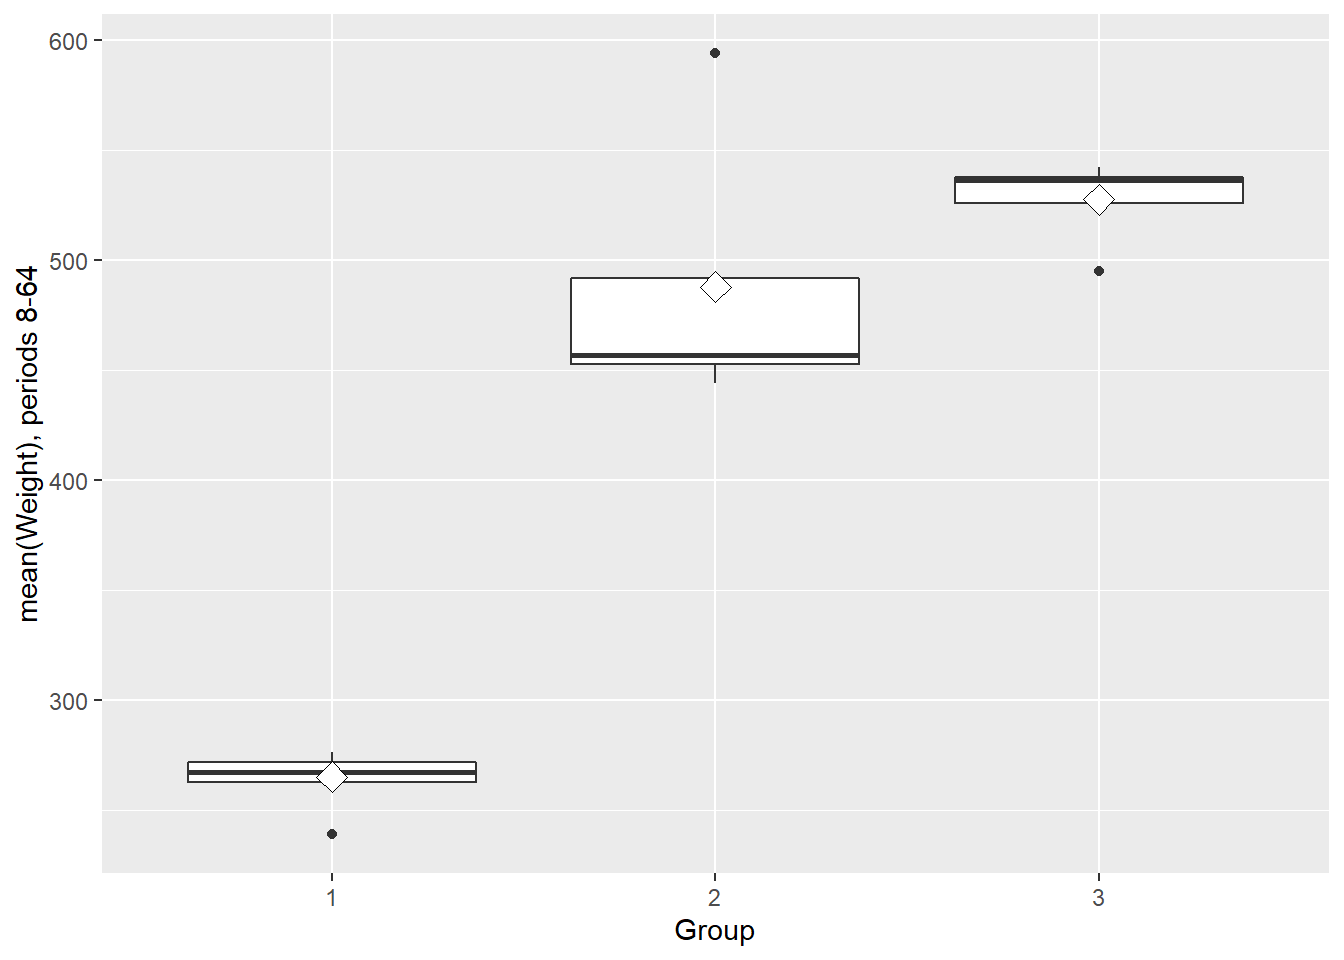
\includegraphics{chapter4_files/figure-latex/unnamed-chunk-8-1.pdf}

\begin{Shaded}
\begin{Highlighting}[]
\CommentTok{# k-means clustering}
\NormalTok{km <-}\KeywordTok{kmeans}\NormalTok{(Boston, }\DataTypeTok{centers=} \DecValTok{2}\NormalTok{)}

\CommentTok{# plot the Boston dataset with clusters}
\KeywordTok{pairs}\NormalTok{(Boston, }\DataTypeTok{col =}\NormalTok{ km}\OperatorTok{$}\NormalTok{cluster)}
\end{Highlighting}
\end{Shaded}

\includegraphics{chapter4_files/figure-latex/unnamed-chunk-8-2.pdf}

\end{document}
